% This file was created by matplotlib2tikz v0.6.18.
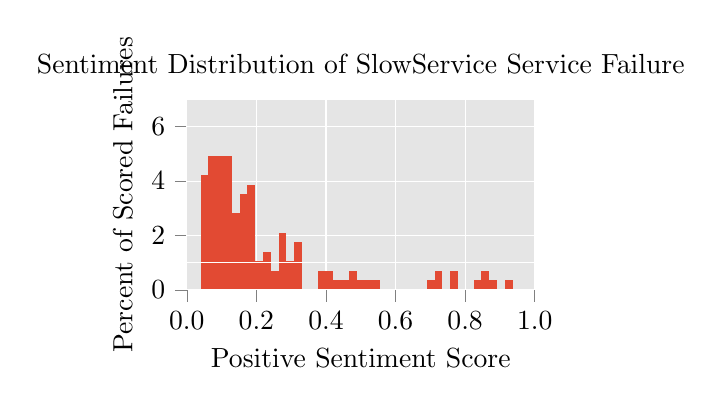
\begin{tikzpicture}

\definecolor{color0}{rgb}{0.886274509803922,0.290196078431373,0.2}

\begin{axis}[
axis background/.style={fill=white!89.80392156862746!black},
axis line style={white},
height=4cm,
tick align=outside,
tick pos=left,
title={Sentiment Distribution of SlowService Service Failure},
width=6cm,
x grid style={white},
xlabel={Positive Sentiment Score},
xmajorgrids,
xmin=0, xmax=1,
xtick={0,0.2,0.4,0.6,0.8,1},
xticklabels={0.0,0.2,0.4,0.6,0.8,1.0},
y grid style={white},
ylabel={Percent of Scored Failures},
ymajorgrids,
ymin=0, ymax=7
]
\draw[fill=color0,draw opacity=0] (axis cs:0.0395509302616119,0) rectangle (axis cs:0.0619783475995064,4.21306597869948);
\draw[fill=color0,draw opacity=0] (axis cs:0.0619783513247967,0) rectangle (axis cs:0.0844057649374008,4.91524364181606);
\draw[fill=color0,draw opacity=0] (axis cs:0.0844057649374008,0) rectangle (axis cs:0.106833182275295,4.91524364181606);
\draw[fill=color0,draw opacity=0] (axis cs:0.106833189725876,0) rectangle (axis cs:0.12926059961319,4.91524364181606);
\draw[fill=color0,draw opacity=0] (axis cs:0.12926059961319,0) rectangle (axis cs:0.151688024401665,2.80870971938884);
\draw[fill=color0,draw opacity=0] (axis cs:0.151688024401665,0) rectangle (axis cs:0.174115434288979,3.51088948193053);
\draw[fill=color0,draw opacity=0] (axis cs:0.174115419387817,0) rectangle (axis cs:0.196542844176292,3.86197586415965);
\draw[fill=color0,draw opacity=0] (axis cs:0.196542859077454,0) rectangle (axis cs:0.218970268964767,1.05326684457916);
\draw[fill=color0,draw opacity=0] (axis cs:0.218970268964767,0) rectangle (axis cs:0.241397693753242,1.40435485969442);
\draw[fill=color0,draw opacity=0] (axis cs:0.241397678852081,0) rectangle (axis cs:0.263825118541718,0.702177429847209);
\draw[fill=color0,draw opacity=0] (axis cs:0.263825118541718,0) rectangle (axis cs:0.286252528429031,2.10653368915832);
\draw[fill=color0,draw opacity=0] (axis cs:0.286252498626709,0) rectangle (axis cs:0.308679908514023,1.05326684457916);
\draw[fill=color0,draw opacity=0] (axis cs:0.308679938316345,0) rectangle (axis cs:0.331107378005981,1.75544240827233);
\draw[fill=color0,draw opacity=0] (axis cs:0.331107378005981,0) rectangle (axis cs:0.353534787893295,0);
\draw[fill=color0,draw opacity=0] (axis cs:0.353534758090973,0) rectangle (axis cs:0.375962167978287,0);
\draw[fill=color0,draw opacity=0] (axis cs:0.375962197780609,0) rectangle (axis cs:0.398389607667923,0.702177896386106);
\draw[fill=color0,draw opacity=0] (axis cs:0.398389607667923,0) rectangle (axis cs:0.420817047357559,0.702176963308932);
\draw[fill=color0,draw opacity=0] (axis cs:0.420817017555237,0) rectangle (axis cs:0.443244427442551,0.351088948193053);
\draw[fill=color0,draw opacity=0] (axis cs:0.443244457244873,0) rectangle (axis cs:0.465671867132187,0.351088948193053);
\draw[fill=color0,draw opacity=0] (axis cs:0.465671837329865,0) rectangle (axis cs:0.488099247217178,0.702177896386106);
\draw[fill=color0,draw opacity=0] (axis cs:0.488099277019501,0) rectangle (axis cs:0.510526716709137,0.351088481654466);
\draw[fill=color0,draw opacity=0] (axis cs:0.510526716709137,0) rectangle (axis cs:0.532954156398773,0.351088481654466);
\draw[fill=color0,draw opacity=0] (axis cs:0.532954216003418,0) rectangle (axis cs:0.555381596088409,0.35108941473288);
\draw[fill=color0,draw opacity=0] (axis cs:0.555381536483765,0) rectangle (axis cs:0.577808976173401,0);
\draw[fill=color0,draw opacity=0] (axis cs:0.577808976173401,0) rectangle (axis cs:0.600236356258392,0);
\draw[fill=color0,draw opacity=0] (axis cs:0.600236356258392,0) rectangle (axis cs:0.622663795948029,0);
\draw[fill=color0,draw opacity=0] (axis cs:0.622663795948029,0) rectangle (axis cs:0.645091235637665,0);
\draw[fill=color0,draw opacity=0] (axis cs:0.64509129524231,0) rectangle (axis cs:0.667518675327301,0);
\draw[fill=color0,draw opacity=0] (axis cs:0.667518615722656,0) rectangle (axis cs:0.689946055412292,0);
\draw[fill=color0,draw opacity=0] (axis cs:0.689946055412292,0) rectangle (axis cs:0.712373495101929,0.351088481654466);
\draw[fill=color0,draw opacity=0] (axis cs:0.712373495101929,0) rectangle (axis cs:0.73480087518692,0.70217882946576);
\draw[fill=color0,draw opacity=0] (axis cs:0.73480087518692,0) rectangle (axis cs:0.757228314876556,0);
\draw[fill=color0,draw opacity=0] (axis cs:0.757228314876556,0) rectangle (axis cs:0.779655754566193,0.702176963308932);
\draw[fill=color0,draw opacity=0] (axis cs:0.779655814170837,0) rectangle (axis cs:0.802083194255829,0);
\draw[fill=color0,draw opacity=0] (axis cs:0.802083134651184,0) rectangle (axis cs:0.82451057434082,0);
\draw[fill=color0,draw opacity=0] (axis cs:0.82451057434082,0) rectangle (axis cs:0.846937954425812,0.35108941473288);
\draw[fill=color0,draw opacity=0] (axis cs:0.846937954425812,0) rectangle (axis cs:0.869365394115448,0.702176963308932);
\draw[fill=color0,draw opacity=0] (axis cs:0.869365394115448,0) rectangle (axis cs:0.891792833805084,0.351088481654466);
\draw[fill=color0,draw opacity=0] (axis cs:0.891792893409729,0) rectangle (axis cs:0.91422027349472,0);
\draw[fill=color0,draw opacity=0] (axis cs:0.914220213890076,0) rectangle (axis cs:0.936647653579712,0.351088481654466);
\path [draw=white, fill opacity=0] (axis cs:0,0)
--(axis cs:0,7);

\path [draw=white, fill opacity=0] (axis cs:1,0)
--(axis cs:1,7);

\path [draw=white, fill opacity=0] (axis cs:0,0)
--(axis cs:1,0);

\path [draw=white, fill opacity=0] (axis cs:0,1)
--(axis cs:1,1);

\end{axis}

\end{tikzpicture}